\section[动量]{动量} \label{sec:03.05} % 
% \makebox[5em][s]{} % 短题目拉间距


动量$\boldsymbol{p}$作为一种力学量,其算符表示为
\eqindent{12}
\begin{empheq}{equation}\label{eq35.1}
	\hat{\boldsymbol{p}}=-i\hbar\nabla
\end{empheq}
如以$\hbar k$表示其本征值,相应的本征函数(暂不考虑归一化问题)为
\begin{empheq}{equation}\label{eq35.2}
	e^{i\boldsymbol{k}\cdot\boldsymbol{r}}=e^{i\boldsymbol{p}\cdot\boldsymbol{r}/\hbar}
\end{empheq}
容易验证,\eqref{eq35.2}式满足本征方程
\begin{empheq}{equation}\label{eq35.3}
	-i\hbar\nabla e^{i\boldsymbol{k}\cdot\boldsymbol{r}}=\hbar\boldsymbol{k}e^{i\boldsymbol{k}\cdot\boldsymbol{r}}
\end{empheq}\eqnormal
而且,只要$k$取实数,则\eqref{eq35.2}式在全空间均取有限值.

{\heiti 1. 连续谱本征函数}

先考虑一维运动,波函数$\varPsi=\varPsi(x)$.以$\boldsymbol{p}=\hbar\boldsymbol{k}$表示见的本征值,$\varPsi_{p}(x)$表示相应的本征函数,满足正交归一化条件[\eqref{eq34.19}式]
\begin{empheq}{equation}\label{eq35.4}
	\int_{-\infty}^{\infty}\varPsi_{p}^{*}(x)\varPsi_{p^{\prime}}(x)dx=\delta(p-p^{\prime})
\end{empheq}
根据$\delta$函数的表示式[参看附录\ref{A01}]
\begin{empheq}{equation}\label{eq35.5}
	\delta(k-k^{\prime})=\frac{1}{2\pi}\int_{-\infty}^{\infty}e^{i(k^{\prime}-k)x}dx
\end{empheq}
以及
\begin{empheq}{equation}\label{eq35.6}
	\delta(k-k^{\prime})=\delta(\hbar k-\hbar k^{\prime})=\frac{1}{\hbar}\delta(k-k^{\prime})
\end{empheq}
易知满足正交归一化条件\eqref{eq35.4}的动量本征函数应该是
\begin{empheq}{equation}\label{eq35.7}
	\varPsi_{p}(x)=\frac{1}{\sqrt{2\pi\hbar}}e^{ipx/\hbar}=\frac{1}{\sqrt{2\pi\hbar}}e^{ikx}
\end{empheq}

任何波函数$\varPsi(x)$可以表示成动量本征函数的线性叠加:
\begin{empheq}{equation}\label{eq35.8}
	\begin{aligned}
		\varPsi(x)&=\int_{-\infty}^{\infty}C(p)\varPsi_{p}(x)dp	\\
		&=\frac{1}{\sqrt{2\pi\hbar}}\int_{-\infty}^{\infty}C(p)e^{ipx/\hbar}dp
	\end{aligned}
\end{empheq}
这相当于\eqref{eq34.17}式.按照\eqref{eq34.20}式,$C(p)$由下式决定:
\begin{empheq}{equation}\label{eq35.9}
	\begin{aligned}
		C(p)&=\int_{-\infty}^{\infty}\varPsi_{p}^{*}(x)\varPsi(x)dx	\\
		&=\frac{1}{\sqrt{2\pi\hbar}}\int_{-\infty}^{\infty}\varPsi(x)e^{-ipx/\hbar}dx
	\end{aligned}
\end{empheq}
\eqref{eq35.8}式和\eqref{eq35.8}式正是数学中的傅里叶变换公式.[参看附录\ref{A01}].

按照波函数的普遍物理诠释,如$\varPsi(x)$已经归一化,则
\eqindent{3}
\begin{empheq}{equation*}
	\boxed{|C(p)|^{2}dp=\text{在$\varPsi$态下$p_{x}$的取值在$(p,p+dp)$范围内的概率}}
\end{empheq}\eqnormal

推广到三维($x,y,z$)运动,动量本征函数取为
\begin{empheq}{equation}\label{eq35.10}
	\varPsi_{\boldsymbol{p}}(\boldsymbol{r})=(2\pi\hbar)^{-\frac{3}{2}}e^{i\boldsymbol{p}\cdot\boldsymbol{r}/\hbar}=(2\pi\hbar)^{-\frac{3}{2}}e^{i\boldsymbol{k}\cdot\boldsymbol{r}}
\end{empheq}
满足正交归—化条件
\eqlong
\begin{empheq}{equation}\label{eq35.11}
	\begin{aligned}
		\int_{\text{全}}\varPsi_{\boldsymbol{p}}^{*}(\boldsymbol{r})\varPsi_{\boldsymbol{p}^{\prime}}(\boldsymbol{r})d\tau	&=(2\pi\hbar)^{-3}\int_{\text{全}}e^{i(\boldsymbol{p}^{\prime}-\boldsymbol{p})\cdot\boldsymbol{r}/\hbar}d\tau
	\end{aligned}
\end{empheq}
任意归一化波函数$\varPsi(\boldsymbol{r})$可以展开成动量本征函数的线性叠加:
\begin{empheq}{equation}\label{eq35.12}
	\begin{aligned}
		\varPsi(\boldsymbol{r})&=\iiint_{-\infty}^{\infty}C(\boldsymbol{p})\varPsi_{\boldsymbol{p}}(\boldsymbol{r})d^{3}p	\\
		&=(2\pi\hbar)^{-\frac{3}{2}}\iiint_{-\infty}^{\infty}C(\boldsymbol{p})e^{i\boldsymbol{p}\cdot\boldsymbol{r}/\hbar}d^{3}p
	\end{aligned}
\end{empheq}
其中
\begin{empheq}{equation}\label{eq35.13}
	\begin{aligned}
		C(\boldsymbol{p})&=\int_{\text{全}}\varPsi_{\boldsymbol{p}}^{*}(\boldsymbol{r})\varPsi(\boldsymbol{r})d\tau	\\
		&=(2\pi\hbar)^{-\frac{3}{2}}\int_{\text{全}}\varPsi(\boldsymbol{r})e^{-\boldsymbol{p}\cdot\boldsymbol{r}/\hbar}d\tau
	\end{aligned}
\end{empheq}\eqnormal
这正是三维傅里叶变换公式.$C(\boldsymbol{p})$的意义是
\eqindent{3}
\begin{empheq}{equation*}
	|C(\boldsymbol{p})|^{2}d^{3}p=\text{在$\varPsi$态下动量的取值在$(p,p+d^{3}p)$范围内的概率}
\end{empheq}\eqnormal

{\heiti 2.“方箱归一化”方法}

为了使动量本征函数可以归一化为1(同时本征值出现量子化),常常使用“方箱归一化” 方法,即设想所有物理过程被限制在一个大箱子$L^{3}\bigg(|x|\geqslant\frac{L}{2},|y|\geqslant\frac{L}{2},|z|\geqslant\frac{L}{2},\bigg)$中进行,最后令$L\rightarrow\infty$,因此实际上并未对物理过程有所限制.

先讨论一维运动,“箱子”范围为$-\frac{L}{2}\geqslant \geqslant\frac{L}{2}$.$\hat{p_{x}}$的本征值记为$p$,归一化的本征函数为
\begin{empheq}{equation}\label{eq35.14}
	\varPsi_{p}(x)=\frac{1}{\sqrt{L}}e^{ipx/\hbar}
\end{empheq}
满足归一化条件
\begin{empheq}{equation}\label{eq35.15}
	\int_{-\frac{L}{2}}^{\frac{L}{2}}\varPsi^{*}\varPsi dx=1
\end{empheq}
为了保证$\hat{p_{x}}=-i\hbar\frac{\partial}{\partial x}$是厄密算符,对于任何$\varPsi_{1}$,$\varPsi_{2}$,应该有[参看(3.2.12)式]
\begin{empheq}{equation*}
	\int_{-\frac{L}{2}}^{\frac{L}{2}}\varPsi_{1}^{*}\hat{p_{x}}\varPsi_{2}dx=-\int_{-\frac{L}{2}}^{\frac{L}{2}}\varPsi_{2}(\hat{p_{x}}\varPsi_{1})^{*}dx
\end{empheq}
亦即
\eqindent{5}
\begin{empheq}{equation*}
	\begin{aligned}
		-\int_{-\frac{L}{2}}^{\frac{L}{2}}\varPsi_{1}^{*}\frac{d}{dx}\varPsi_{2}dx
		&=\int_{-\frac{L}{2}}^{\frac{L}{2}}\varPsi_{2}\frac{d}{dx}\varPsi_{1}^{*}dx	\\
		&=\varPsi_{2}\varPsi_{1}^{*}\bigg|_{-\frac{L}{2}}^{\frac{L}{2}}-\int_{-\frac{L}{2}}^{\frac{L}{2}}\varPsi_{1}^{*}\frac{d}{dx}\varPsi_{2}dx
	\end{aligned}
\end{empheq}\eqnormal
为此必须
\begin{empheq}{equation}\label{eq35.16}
	\varPsi_{1}^{*}\bigg(-\frac{L}{2}\bigg)\varPsi_{2}\bigg(-\frac{L}{2}\bigg)=\varPsi_{1}^{*}\bigg(\frac{L}{2}\bigg)\varPsi_{2}\bigg(\frac{L}{2}\bigg)
\end{empheq}
取$\varPsi_{1}(x)=1$,$\varPsi_{2}(x)=\varPsi(x)$,\eqref{eq35.16}式成为
\begin{empheq}{equation}\label{eq35.17}
	\varPsi\bigg(-\frac{L}{2}\bigg)=\varPsi\bigg(\frac{L}{2}\bigg)
\end{empheq}
称为周期性边界条件.这是为了保证$\hat{p_{x}}$是厄密算符,波函数必须满足的条件.令$\varPsi_{p}(x)$满足周期性边界条件\eqref{eq35.17},即得
\eqindent{12}
\begin{empheq}{equation}\label{eq35.18}
	e^{ipL/\hbar}=1
\end{empheq}\eqnormal
这是“箱归一化”对动量本征值$p$带来的限制条件,即量子化条件.满足\eqref{eq35.18}式的动量值是
\begin{empheq}{equation}\label{eq35.19}
	p_{n}=\frac{2\pi n\hbar}{L}=\frac{nh}{L},\quad n=0,\pm 1,\pm 2,\cdots
\end{empheq}
相应的归一化本征函数为
\begin{empheq}{equation}\label{eq35.20}
	\varPsi_{n}(x)=\frac{1}{\sqrt{L}}e^{ip_{n}x/\hbar}=\frac{1}{\sqrt{L}}e^{i2\pi nx/L}
\end{empheq}
它们显然满足正交归一化条件
\begin{empheq}{equation}\label{eq35.21}
	\int_{-\frac{L}{2}}^{\frac{L}{2}}\varPsi_{n}^{*}(x)\varPsi_{n^{\prime}}(x)dx=\delta_{nn^{\prime}}
\end{empheq}
以及完备性条件
\begin{empheq}{equation}\label{eq35.22}
	\sum_{n}\varPsi_{n}(x)\varPsi_{n}^{*}(x^{\prime})=\sum_{n=-\infty}^{\infty}\frac{1}{L}e^{i2\pi n(x-x^{\prime})/L}
\end{empheq}

任何满足周期性边界条件\eqref{eq35.17}式(注意,$x=\pm\frac{L}{2}$处如$\varPsi\rightarrow 0$,就属这种情形)的波函数$\varPsi$总可以表示成\eqref{eq35.20}式的线性叠加:
\begin{empheq}{equation}\label{eq35.23}
	\varPsi(x)=\sum_{n}C_{n}\varPsi_{n}(x)=\frac{1}{\sqrt{L}}\sum_{n}C_{n}e^{ip_{n}x/\hbar}
\end{empheq}
其中
\begin{empheq}{equation}\label{eq35.24}
	\begin{aligned}
		C_{n}&=\int_{-\frac{L}{2}}^{\frac{L}{2}}\varPsi_{n}^{*}(x)\varPsi(x)dx	\\
		&=\frac{1}{\sqrt{L}}\int_{-\frac{L}{2}}^{\frac{L}{2}}\varPsi(x)e^{-2\pi nx/L}
	\end{aligned}
\end{empheq}
这正是以$L$为周期的任意函数$\varPsi(x)$的傅里叶级数展开式.将以上公式和连续谱公式比较,可以归纳出以下对应规则:
\eqindent{5}
\begin{empheq}{equation}\label{eq35.25}
	\sum_{n} —— \int dp,\quad \delta_{nn^{\prime}} —— \delta(p-p^{\prime}),\quad \frac{1}{\sqrt{L}} —— \frac{1}{\sqrt{h}}
\end{empheq}\eqnormal
推广到三维情况,$\varPsi=\varPsi(x,y,z)$,为了保证$\hat{p_{x}},\hat{p_{y}},\hat{p_{z}}$为厄密算符,波函数必须满足周期性边界条件:
\begin{empheq}{equation}\label{eq35.26}
	\varPsi(x,y,z)\bigg|_{x=-\frac{L}{2}}^{x=\frac{L}{2}}=0,\quad y,z\text{类似}
\end{empheq}
由此求得动量本征值为
\begin{empheq}{equation}\label{eq35.27}
	\begin{aligned}
		&p_{x}=\frac{n_{1}h}{L},\quad p_{y}=\frac{n_{2}h}{L},\quad p_{z}=\frac{n_{3}h}{L}	\\
		&n_{1},n_{2},n_{3}=0,\pm 1,\pm 2,\pm 3\cdots
	\end{aligned}
\end{empheq}
相应的归一化本征函数为
\begin{empheq}{equation}\label{eq35.28}
	\begin{aligned}
		\varPsi_{p}(\boldsymbol{r})&=\varPsi_{n_{1}n_{2}n_{3}}(x,y,z)=L^{-\frac{3}{2}}e^{i\boldsymbol{p}\cdot\boldsymbol{r}/\hbar}	\\
		&=L^{-\frac{3}{2}}\exp^{i2\pi(n_{1}x+n_{2}y+n_{3}z)/L}
	\end{aligned}
\end{empheq}
满足正交归一化条件
\eqindent{6}
\begin{empheq}{equation}\label{eq35.29}
	\int_{L^{3}}\varPsi_{n_{1}n_{2}n_{3}}^{*}(\boldsymbol{r})\varPsi_{n_{1\prime}n_{2\prime}n_{3\prime}}(\boldsymbol{r})d\tau=\delta_{n_{1}n_{1}^{\prime}}\delta_{n_{2}n_{2}^{\prime}}\delta_{n_{3}n_{3}^{\prime}}
\end{empheq}
以及完备性条件
\begin{empheq}{equation}\label{eq35.30}
	\sum_{n_{1},n_{2},n_{3}}\varPsi_{n_{1}n_{2}n_{3}}(\boldsymbol{r})\varPsi_{n_{1}n_{2}n_{3}}^{*}(\boldsymbol{r^{\prime}})=\delta(\boldsymbol{p}-\boldsymbol{p^{\prime}})
\end{empheq}\eqnormal
满足周期性边界条件\eqref{eq35.26}的任意波函数$\varPsi(\boldsymbol{r})$可以展开为\eqref{eq35.28}式的线性叠加:
\begin{empheq}{equation}\label{eq35.31}
	\varPsi(\boldsymbol{r})=\sum_{n_{1},n_{2},n_{3}}C_{n_{1}n_{2}n_{3}}\varPsi_{n_{1}n_{2}n_{3}}(\boldsymbol{r})
\end{empheq}
其中
\begin{empheq}{equation}\label{eq35.32}
	C_{n_{1}n_{2}n_{3}}=\int_{L^{3}}\varPsi_{n_{1}n_{2}n_{3}}^{*}(\boldsymbol{r})\varPsi(\boldsymbol{r})d\tau
\end{empheq}
和连续谱的对应过渡规则为
\begin{empheq}{equation}\label{eq35.33}
	\begin{aligned}
		&\sum_{n_{1},n_{2},n_{3}} —— \iiint d^{3}p,\quad L^{-\frac{3}{2}}\qquad h^{-\frac{3}{2}}	\\
		&\delta_{n_{1}n_{1}^{\prime}}\delta_{n_{2}n_{2}^{\prime}}\delta_{n_{3}n_{3}^{\prime}} —— \delta(\boldsymbol{p}-\boldsymbol{p^{\prime}})
	\end{aligned}
\end{empheq}

在“箱归一化”方法中,$n_{1},n_{2},n_{3}$的变化单位为1,$p_{x},p_{y},p_{z}$的变化单位为$\frac{h}{L}$,当$L\rightarrow\infty$,$\boldsymbol{p}$的变化就可以当作连续变化.在$(p_{x},p_{x}+dp_{x})$范围内,$p_{x}$共有$\frac{Ldp_{x}}{h}$种不同取值,亦即有$\frac{Ldp_{x}}{h}$种动量本征态.则在$d^{3}p=dp_{x}dp_{y}dp_{z}$范围内,本征态数目为
\eqindent{12}
\begin{empheq}{equation}\label{eq35.34}
	\frac{L^{3}d^{3}p}{\hbar^{3}}
\end{empheq}\eqnormal
或者说,“相空间”(坐标-动量六维空间)每$h^{3}$范围内平均存在一个动量本征态.

\begin{wrapfigure}[6]{r}{7em}
	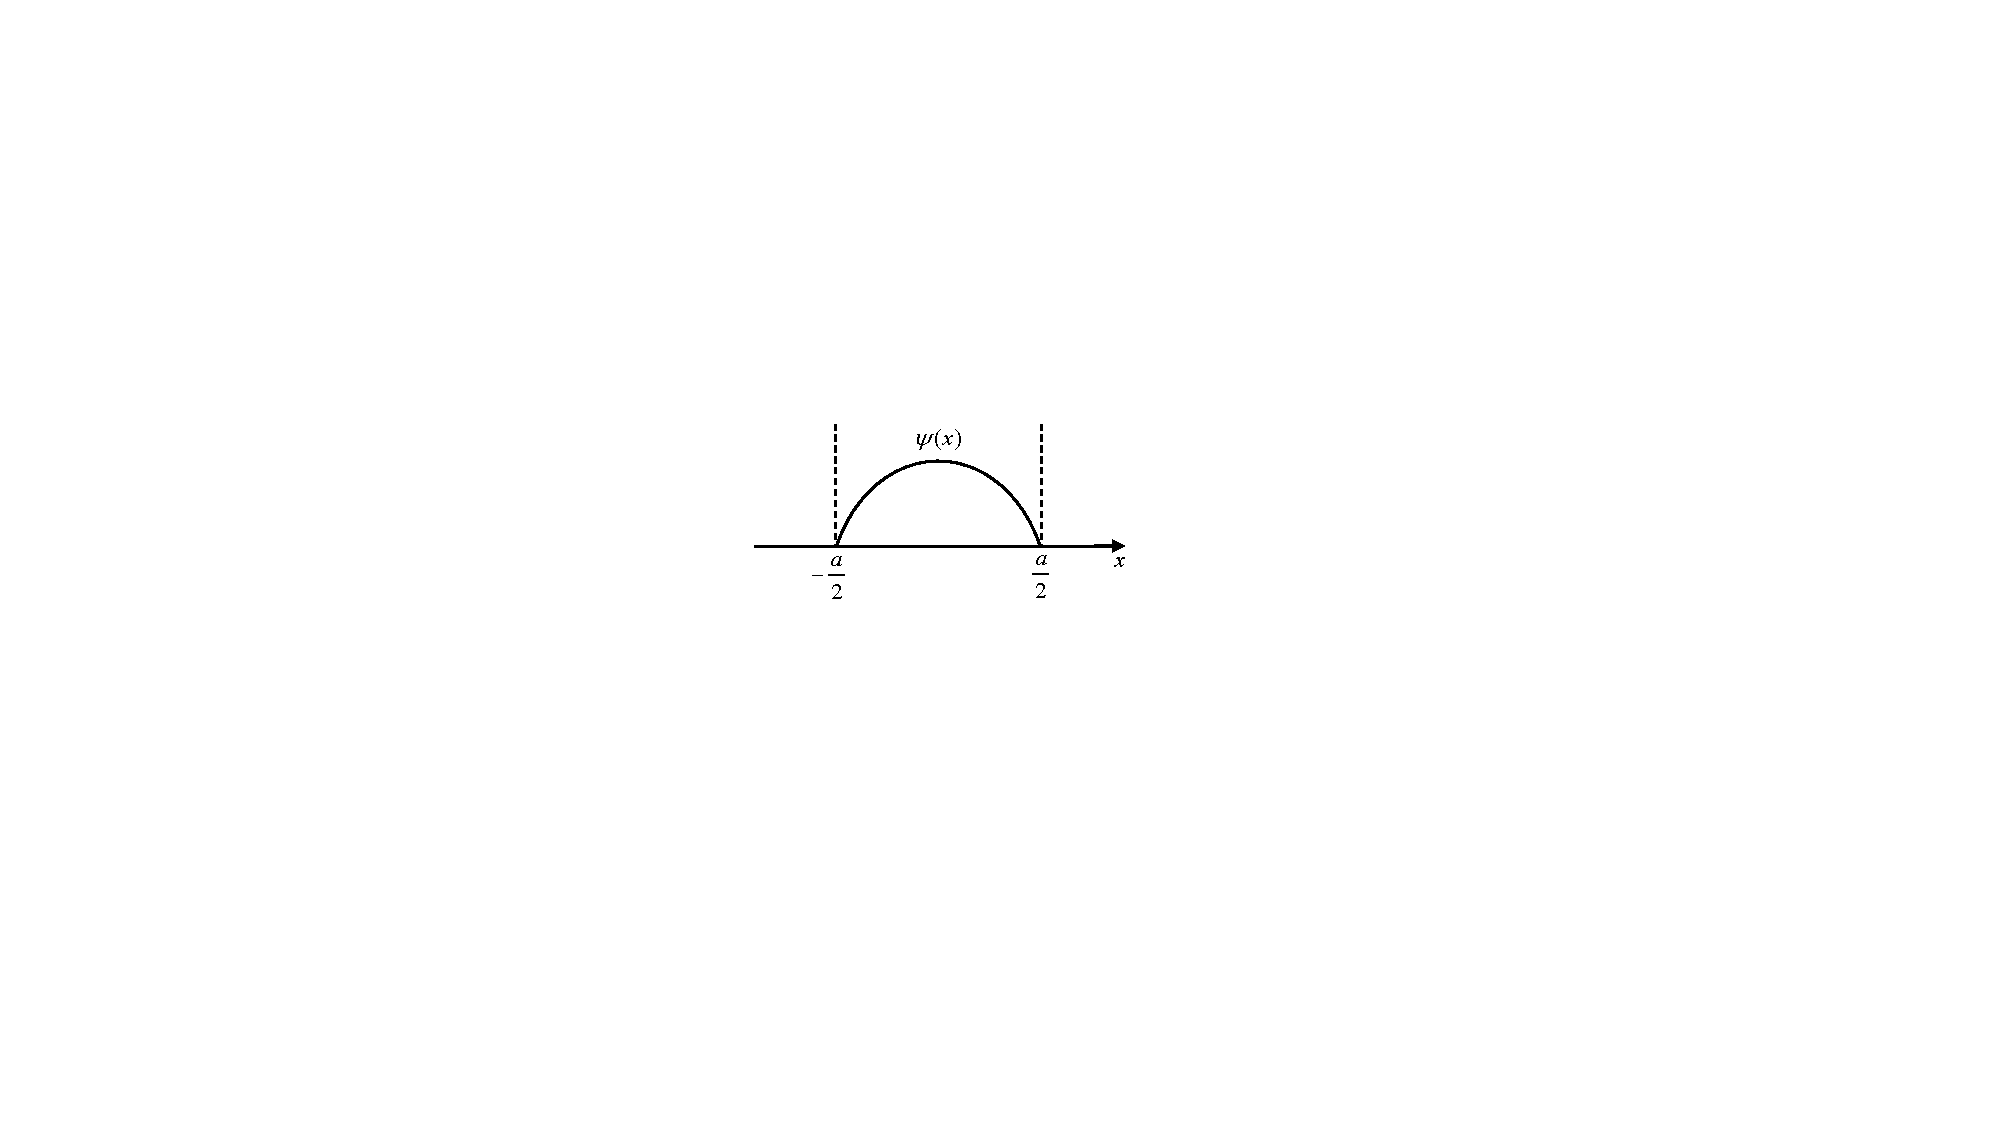
\includegraphics[width=3.5cm]{QM file/figure/3-1}
	\caption{}\label{fig.3-1}
\end{wrapfigure}

\example 如图\ref{fig.3-1},粒子在无限深势阱$\bigg(-\frac{a}{2}<x<\frac{a}{2}\bigg)$中运动,处于基态.如果突然破除势“墙”,而让粒子自由运动,粒子随即在一个方向(例如在$x>\frac{a}{2}$方向)被测量.设测得粒子动能在$(E,E+dE)$范围内的几率为$w(E)dE$,求$w(E)$.

\solution 势“墙”刚破除时,粒子的波函数$\varPsi(x)$就是势阱中的基态波函数,(波函数随时间的变化是连续的,不会突变.)根据\eqref{eq24.10}式,可知
\begin{empheq}{equation}\label{eq35.35}
	\varPsi(x)=
	\begin{dcases}
		\sqrt{\frac{2}{a}}\cos\frac{\pi x}{a},	& |x|<\frac{a}{2}	\\
		0,	& |x|>\frac{a}{2}
	\end{dcases}
\end{empheq}
势“墙”破除后,粒子将在全空间($-\infty<x<\infty$)自由运动.将$\varPsi(x)$展开成动量本征函数的线性叠加:
\begin{empheq}{equation}\label{eq35.36}
	\begin{aligned}
		\varPsi(x)&=\frac{1}{\sqrt{2\pi\hbar}}\int_{-\infty}^{\infty}C(p)e^{ipx/\hbar}dp	\\
		&=\frac{1}{\sqrt{2\pi}}\int_{-\infty}^{\infty}C(k)e^{ikx}dk
	\end{aligned}
\end{empheq}
其中
\begin{empheq}{equation}\label{eq35.37}
	p=\hbar k,\quad dp=\hbar dk,\quad C(k)=\sqrt{\hbar}C(p)
\end{empheq}
按照概率诠释,

$|C(k)|^{2}dk=|C(p)|^{2}dp=$粒子动量在$(p,p+dp)$范围内的概率,粒子自由运动时,能量(动能)和动量的关系是
\begin{empheq}{equation}\label{eq35.38}
	\begin{aligned}
			E	&=\frac{p^{2}}{2m}=\frac{\hbar^{2}k^{2}}{2m}	\\
		dE	&=\frac{\hbar^{2}kdk}{m}
	\end{aligned}
\end{empheq}
因此,
\begin{empheq}{equation*}
	w(E)dE=|C(k)|^{2}dk
\end{empheq}
\begin{empheq}{equation}\label{eq35.39}
	w(E)=|C(k)|^{2}\frac{dk}{dE}=\frac{m|C(k)|^{2}}{\hbar^{2}k}
\end{empheq}
可见关键是求出$C(k)$.按照\eqref{eq35.9}式及\eqref{eq35.37}式、\eqref{eq35.35}式,得
\begin{empheq}{equation}\label{eq35.40}
	\begin{aligned}
		C(k)&=\frac{1}{\sqrt{2\pi}}\int_{-\infty}^{\infty}\varPsi(x)e^{-ikx}dx	\\
		&=\frac{1}{\sqrt{\pi a}}\int_{-\frac{a}{2}}^{\frac{a}{2}}e^{-ikx}\cos\frac{\pi x}{a}dx	\\
		&=\sqrt{\frac{a}{\pi}}\bigg(\frac{1}{\pi-ak}+\frac{1}{\pi+ak}\bigg)\cos\frac{ak}{2}
	\end{aligned}
\end{empheq}
\begin{empheq}{equation}\label{eq35.41}
	|C(k)|^{2}=\frac{4\pi a}{(a^{2}k^{2}-\pi^{2})}\cos^{2}\frac{ak}{2}
\end{empheq}
$\dfrac{|C(k)|^{2}}{\hbar}$就是动量的概率分布函数$|C(p)|^{2}$,$|C(k)|^{2}$随$k$的变化如表\ref{lab.3-1}和图\ref{fig.3-2}所示

\begin{table}[!h]
	\begin{center}
		\caption{}\label{lab.3-1}
		\begin{tabular}{c|c|c|c|c|c|c|c|c}
			\hline 
			\multirow{2}{*}{$\dfrac{ka}{\pi}$} & \multirow{2}{*}{0} & \multirow{2}{*}{0.5} & \multirow{2}{*}{1} & \multirow{2}{*}{1.5} & \multirow{2}{*}{2} & \multirow{2}{*}{3} & \multirow{2}{*}{3.779} & \multirow{2}{*}{5} \\ 
			& & & & & & & & \\ \hline
			\multirow{2}{*}{$|C(k)|^{2}$} & \multirow{2}{*}{$\dfrac{4a}{\pi^{3}}$} & \multirow{2}{*}{$\dfrac{32a}{9\pi^{3}}$} & \multirow{2}{*}{$\dfrac{a}{4\pi}$} & \multirow{2}{*}{$\dfrac{32a}{25\pi^{3}}$} & \multirow{2}{*}{$\dfrac{4}{9\pi^{3}}$} & \multirow{2}{*}{0} & \multirow{2}{*}{\text{(极大)}} & \multirow{2}{*}{0} \\ 
			& & & & & & & & \\ \hline
			\multirow{2}{*}{$|\dfrac{C(k)}{C(0)}|^{2}$} & \multirow{2}{*}{1} & \multirow{2}{*}{$\dfrac{8}{9}$} & \multirow{2}{*}{$\dfrac{\pi^{2}}{16}$} & \multirow{2}{*}{$\dfrac{8}{25}$} & \multirow{2}{*}{$\dfrac{1}{9}$} & \multirow{2}{*}{0} & \multirow{2}{*}{0.005} & \multirow{2}{*}{0} \\ 
			& & & & & & & & \\ \hline
		\end{tabular}
	\end{center}
\end{table}

由图3-2可见,动量分布概率绝大部分集中在$|ka|<2\pi$范围内.如按下式粗略地规定(这样便于计算)分布半宽$\Delta k$,
\begin{empheq}{equation*}
	|C(0)|^{2}2\Delta k=\int_{-\infty}^{\infty}|C(k)|^{2}dk=1
\end{empheq}
则
\begin{empheq}{equation}\label{eq35.42}
	\frac{a}{\hbar}\Delta k=\frac{\pi^{2}}{8}=\num{1.23},\quad\Delta k=\num{1.23}\frac{\pi}{a}
\end{empheq}

\begin{figure}[!h]
	\centering
	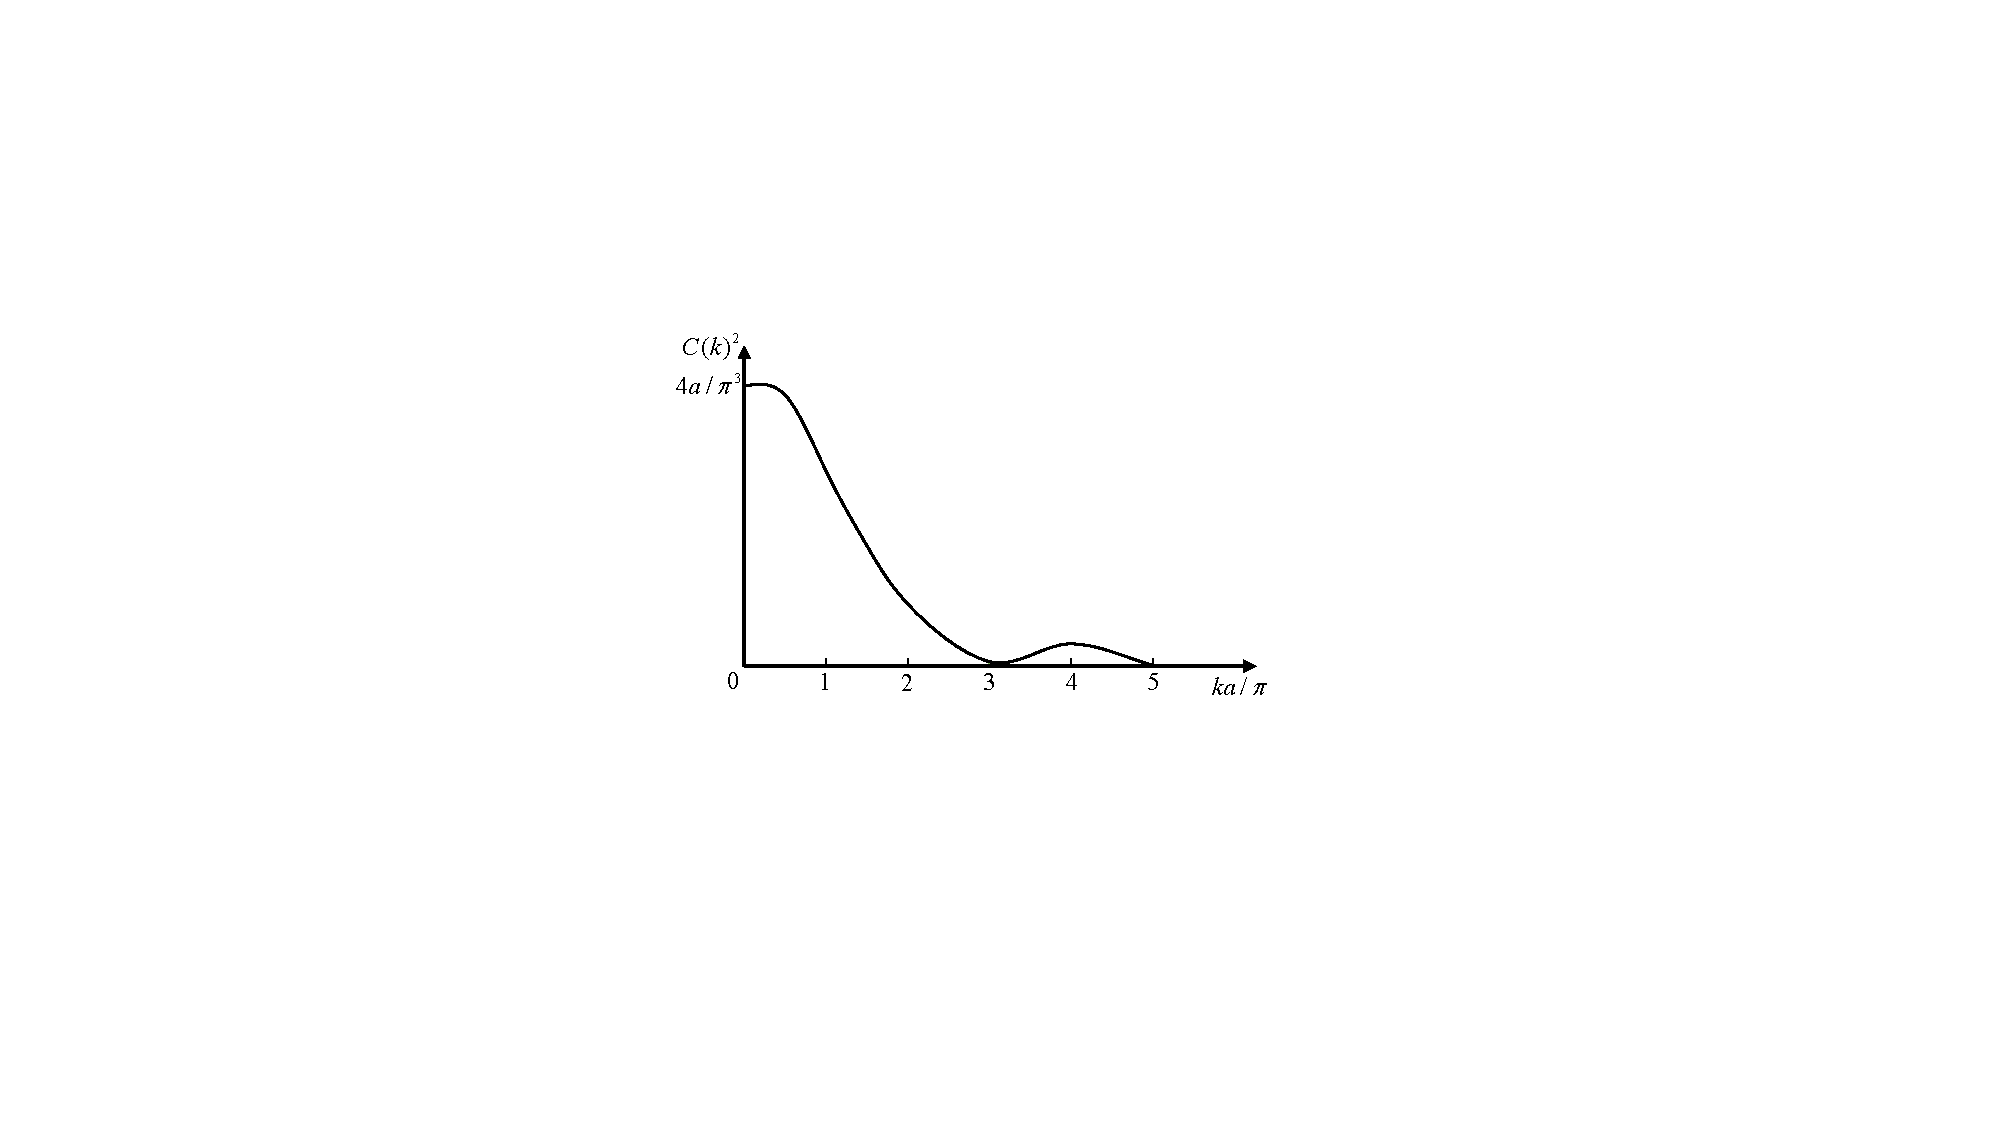
\includegraphics[width=5cm,clip]{QM file/figure/3-2}
	\caption{}\label{fig.3-2}
\end{figure}
$\Delta k$和波函数\eqref{eq35.35}式中的$k=\dfrac{\pi}{a}$很接近.

由\eqref{eq35.39}、\eqref{eq35.41}式求得粒子的动能概率分布函数为
\eqindent{5}
\begin{empheq}{equation}\label{eq35.43}
	\begin{aligned}
		w(E)&=\frac{m}{\hbar^{2}k}\frac{4\pi a}{(a^{2}k^{2}-\pi^{2})}\cos^{2}\frac{ak}{2}	\\
		&=\frac{1}{\hbar}\sqrt{\frac{m}{2E}}\frac{4\pi a}{\bigg(\frac{a^{2}}{\hbar^{2}}2mE-\pi^{2}\bigg)^{2}}\cos^{2}\frac{a}{\hbar}\sqrt{\frac{mE}{2}}
	\end{aligned}
\end{empheq}\eqnormal
用围道积分法不难验证:
\begin{empheq}{equation}\label{eq35.44}
	2\int_{0}^{\infty}w(E)dE=\int_{-\infty}^{\infty}|C(k)|^{2}dk=1
\end{empheq}

